\documentclass[12pt,a4paper]{article}

\usepackage{fontspec}
\defaultfontfeatures{Ligatures=TeX}
\usepackage{polyglossia}
\setdefaultlanguage{russian}
\setotherlanguage{english}
\setmainfont{Times New Roman}
\setsansfont{Arial}
\setmonofont{Courier New}
\newfontfamily\cyrillicfont{Times New Roman}
\newfontfamily\cyrillicfontsf{Arial}
\newfontfamily\cyrillicfonttt{Courier New}
\usepackage{amsmath,amssymb,amsfonts}
\usepackage{amsthm}
\usepackage[margin=2.5cm]{geometry}
\usepackage[numbers,sort&compress]{natbib}
\usepackage{microtype}
\usepackage{hyperref}

\tolerance=1500
\emergencystretch=1.5em
\usepackage{xcolor}
\usepackage{booktabs}
\usepackage{mathtools}
\usepackage[shortlabels]{enumitem}
\usepackage{graphicx}
\usepackage{doi}
\usepackage{tikz}
\usetikzlibrary{arrows.meta,positioning}

\newtheorem{theorem}{Теорема}[section]
\newtheorem{lemma}[theorem]{Лемма}
\newtheorem{corollary}[theorem]{Следствие}
\newtheorem{proposition}[theorem]{Утверждение}
\newtheorem{conjecture}[theorem]{Гипотеза}
\theoremstyle{definition}
\newtheorem{definition}[theorem]{Определение}
\theoremstyle{remark}
\newtheorem{remark}[theorem]{Замечание}

%%% Custom commands
\newcommand{\Weylsq}{C_{\mu\nu\rho\sigma}C^{\mu\nu\rho\sigma}}
\newcommand{\dualCC}{\!{}^{\ast}\!C_{\mu\nu}{}^{\rho\sigma}C_{\rho\sigma}{}^{\mu\nu}}
\newcommand{\dd}{\mathrm{d}}
\newcommand{\Tr}{\operatorname{Tr}}
\newcommand{\tr}{\operatorname{tr}}
\newcommand{\half}{\tfrac{1}{2}}
\newcommand{\Lam}{\Lambda}
\newcommand{\order}{\mathcal{O}}
\newcommand{\SD}{\mathrm{SD}}
\newcommand{\ASD}{\mathrm{ASD}}

\hypersetup{
  colorlinks=true,
  linkcolor=blue!60!black,
  citecolor=blue!60!black,
  urlcolor=blue!60!black,
  pdfauthor={Давид Алфёров},
  pdftitle={Киральность коэффициентов Сили--Де~Витта и квартичная вейлевская структура в спектральном действии},
  pdfsubject={hep-th}
}

\begin{document}

\title{Киральность коэффициентов Сили--Де~Витта и квартичная вейлевская
структура в спектральном действии}

\author{Давид Алфёров\\[4pt]
\small Независимый исследователь, Россия\\[2pt]
\small\textit{davidich.alfyorov@gmail.com}}

\date{Март 2026}

\maketitle

% ============================================================
\begin{abstract}
% ============================================================

Мы доказываем, что свёрнутые коэффициенты Сили--Де~Витта $\tr(a_{2n})$ для
оператора Дирака на Риччи-плоском четырёхмерном многообразии разлагаются как
$\tr(a_{2n}) = f_n(p) + f_n(q)$, где $p = |C^+|^2$ и $q = |C^-|^2$ ---
квадраты норм самодуального и антисамодуального тензоров Вейля.
Доказательство опирается на \emph{теорему о киральности}: генераторы
спинорной связности $\sigma^{rs} = \frac{1}{4}[\gamma^r, \gamma^s]$
коммутируют с оператором киральности $\gamma_5$ в четырёх измерениях, что
делает эндоморфизм кривизны $\Omega_{\mu\nu}$ блочно-диагональным в
киральном базисе.  Мы устанавливаем \emph{перекрёстное киральное
соответствие} --- левый спинорный блок связывается исключительно с
антисамодуальным тензором Вейля, а правый блок --- с самодуальной
частью --- с помощью разложения по символам 'т~Хоофта.  На квартичном
уровне (массовая размерность~8) теорема означает, что $\tr(a_8)$ содержит
только комбинацию $c(p^2 + q^2)$ с нулевым перекрёстным членом $pq$,
фиксируя соотношение $(C^2)^2 : (\!{}^{\ast}\!CC)^2 = 1{:}1$ точно.
Результат распространяется на полную спектральную тройку Стандартной модели
на почти коммутативной геометрии $M \times F$.  С помощью анализа ряда
Мольена три P-чётных квартичных вейлевских инварианта
сначала сводятся к двум посредством тождества Кэли--Гамильтона, а затем к
одной эффективной структуре благодаря киральности.  Это сводит задачу
трёхпетлевой конечности для спектрального действия от переопределённой
системы к одному условию на соотношение.  Мы показываем, что строгая
гипотеза о спектральной перенормируемости для гравитации
\emph{исключена на уровне структурного анализа}: пропагатор гравитона является слепым к киральности
(скаляром в поперечно-бесследовом секторе), а суммы по нескольким собственным значениям на
двух петлях и выше порождают перекрёстные члены $pq$ вне пространства
спектральных функций.  Точное препятствие состоит в многоследовой
структуре разделённых разностей в подходе ван~Нуланда--ван~Сёйлекома,
применённом к гравитации, где метрика изменяет сам оператор Дирака, а не
входит как внутренняя флуктуация.  Тем не менее нарушение количественно
пренебрежимо: перекрёстные члены подавлены множителем
$\alpha_C^3/(16\pi^2)^3 \approx 3{,}2 \times 10^{-10}$, и спектральное
действие обеспечивает эффективную ультрафиолетовую конечность в
пертурбативном режиме с данной точностью.  Все алгебраические результаты
верифицированы независимым численным вычислением на ансамблях случайных
тензоров Вейля с точностью $\leq 10^{-12}$.
\end{abstract}

\noindent\textbf{PACS:} 04.60.-m, 04.62.+v, 11.10.Gh, 02.40.Gh

\tableofcontents
\newpage


% ============================================================
\section{Введение}
\label{sec:intro}
% ============================================================

Принцип спектрального действия~\cite{Chamseddine:1996zu,Chamseddine:2006ep}
кодирует всю бозонную динамику гравитации и калибровочных полей в спектре
оператора Дирака: $S = \Tr\, f(D^2/\Lam^2)$, где $D$ --- оператор Дирака
некоммутативной геометрии, $\Lam$ --- спектральное обрезание, а $f$ ---
положительная чётная функция.  Асимптотическое разложение этого следа по
коэффициентам Сили--Де~Витта~\cite{DeWitt:1964mxt,Gilkey:1975iq,%
Vassilevich:2003xt} воспроизводит действие Эйнштейна--Гильберта,
космологическую постоянную и члены Янга--Миллса Стандартной
модели~\cite{Chamseddine:2010ud,vanSuijlekom:2014pya}, тогда как нелокальное
расширение порождает зависящие от импульса формфакторы, характеризующие
однопетлевое квантово-гравитационное эффективное
действие~\cite{Barvinsky:1985an,Barvinsky:1987uw,Codello:2012kq}.

Киральное разложение спинорной связности в четырёх измерениях является
классическим результатом дифференциальной геометрии и математической физики.
Эгучи, Гилки и Хэнсон~\cite{EguchiGilkeyHanson:1980} установили
блочно-диагональную структуру спинорной кривизны в своём обзоре
гравитационных инстантонов.  То же разложение лежит в основе теоремы
об индексе Атьи--Зингера в четырёх измерениях и широко используется в
самодуальной гравитации и физике
инстантонов~\cite{AtiyahSinger:1968,AlvarezGaume:1983ig}.
В контексте спектрального действия Шамседдин, Конн и
Марколли~\cite{ChamseddineConnesMarcolli:2007} вычислили полное действие
Стандартной модели из принципа спектрального действия на произведении
геометрий $M \times F$, а ван~Сёйлеком~\cite{vanSuijlekom:2014pya}
систематически изложил разложение ядра теплопроводности.

Новизна настоящей работы состоит не в киральности генераторов спинорной
связности (которая является классической), а в систематическом применении
этого свойства к квартичной вейлевской структуре спектрального действия.
Мы показываем, что киральное блочно-диагональное разложение в сочетании с
тождеством Кэли--Гамильтона для вейлевских спиноров сводит пространство
квартичных вейлевских инвариантов от трёх (счёт Мольена) к одной
эффективной структуре, точно соответствующей единственному спектральному
параметру.  Это разрешает видимую переопределённость задачи трёхпетлевой
конечности.

Однопетлевые формфакторы спектрального действия с полным содержанием
Стандартной модели --- дающие $\alpha_C = 13/120$ и
$\alpha_R(\xi) = 2(\xi - 1/6)^2$ --- вычислены
в~\cite{Alfyorov:2026ff}, а наблюдательные следствия (нижняя граница
$\Lam > 2{,}565 \times 10^{-3}\;\mathrm{eV}$) выведены
в~\cite{Alfyorov:2026ss}.

Эти результаты устанавливают пертурбативную конечность на одной петле
(степень расходимости $D = 0$) и, путём явного вычисления на массовой
оболочке, на двух петлях~\cite{Goroff:1985th,Stelle:1976gc}.  Однако на трёх
петлях контрчлен при квадрате кривизны включает квартичные вейлевские
инварианты массовой размерности~8.  Ряд Мольена для кольца инвариантов
$\mathrm{SO}(4)$, действующего на тензоре Вейля, даёт три P-чётных квартичных инварианта, сводящихся к двум по тождеству
Кэли--Гамильтона для бесследовых симметричных $3 \times 3$
самодуальных и антисамодуальных вейлевских
спиноров~\cite{Fulling:1992vm}.  Спектральное действие предоставляет единственный
подстраиваемый параметр ($\delta f_8$, восьмой момент спектральной функции),
что приводит к видимо переопределённой системе: два независимых инварианта
против одного параметра.

В данной работе мы доказываем, что переопределение разрешается свойством
киральности, внутренне присущим оператору Дирака в четырёх измерениях.
Основной результат:

\begin{theorem}[Теорема о киральности --- неформальная формулировка]
\label{thm:informal}
На Риччи-плоском четырёхмерном многообразии коэффициенты Сили--Де~Витта
$\tr(a_{2n})$ лапласиана Дирака $D^2 = -\nabla^2_{\mathrm{spin}}$
имеют вид $f_n(p) + f_n(q)$ при всех порядках~$n$, где
$p = |C^+|^2$, $q = |C^-|^2$.  В частности, $\tr(a_8) = c(p^2 + q^2)$
с нулевым перекрёстным членом $pq$, что сводит эффективное квартичное
вейлевское содержание спектрального действия к единственной структуре.
\end{theorem}

\noindent Теорема применима к полной спектральной тройке Стандартной модели на
произведении геометрий $M \times F$ и имеет прямые следствия для программы
трёхпетлевой конечности.

\medskip
\noindent\textbf{Структура работы.}
В разделе~\ref{sec:notation} фиксируются обозначения.
В разделе~\ref{sec:chirality} формулируется и доказывается теорема о
киральности.  В разделе~\ref{sec:crossed} устанавливается перекрёстное
киральное соответствие посредством символов 'т~Хоофта.
В разделе~\ref{sec:heat} выводится разложение ядра теплопроводности и
результат о нулевом $pq$ на квартичном уровне.
В разделе~\ref{sec:sm} результат распространяется на полную спектральную
тройку Стандартной модели.  В разделе~\ref{sec:quartic} проводится численный
анализ трёх квартичных $\Omega$-структур.
В разделе~\ref{sec:molien} выполняется подсчёт инвариантов с помощью ряда
Мольена.  В разделе~\ref{sec:threeloop} обсуждаются следствия для
трёхпетлевой конечности.  В разделе~\ref{sec:conjecture} формулируется
гипотеза о спектральной перенормируемости.
В разделе~\ref{sec:numerical} приводится программа численной верификации.
В разделе~\ref{sec:conclusions} даётся заключение.

Соглашения: мы работаем в евклидовой сигнатуре $(+,+,+,+)$ на протяжении
всей работы, с алгеброй Клиффорда $\{\gamma^a, \gamma^b\} = 2\delta^{ab}$,
и используем натуральные единицы $c = \hbar = 1$.


% ============================================================
\section{Обозначения и соглашения}
\label{sec:notation}
% ============================================================

\subsection{Алгебра Клиффорда и киральность}

Пусть $(M^4, g)$ --- замкнутое риманово четырёхмерное многообразие.
Евклидова алгебра Клиффорда порождается матрицами $\gamma^a$
($a = 0,1,2,3$), удовлетворяющими
\begin{equation}\label{eq:clifford}
  \{\gamma^a, \gamma^b\} = 2\,\delta^{ab}\,\mathbf{1}_4\,.
\end{equation}
В киральном представлении
\begin{equation}
  \gamma^j = \begin{pmatrix} 0 & -i\sigma_j \\ i\sigma_j & 0 \end{pmatrix}
  \quad (j = 0,1,2), \qquad
  \gamma^3 = \begin{pmatrix} 0 & \mathbf{1}_2 \\ \mathbf{1}_2 & 0 \end{pmatrix},
\end{equation}
где $\sigma_j$ --- матрицы Паули.  Оператор киральности равен
\begin{equation}\label{eq:g5}
  \gamma_5 \;=\; \gamma^0 \gamma^1 \gamma^2 \gamma^3
  \;=\; \begin{pmatrix} \mathbf{1}_2 & 0 \\ 0 & -\mathbf{1}_2 \end{pmatrix},
\end{equation}
и удовлетворяет $\gamma_5^2 = \mathbf{1}_4$, $\gamma_5^\dagger = \gamma_5$,
$\{\gamma_5, \gamma^a\} = 0$ для всех~$a$.  Киральные проекторы определяются
как
\begin{equation}
  P_L = \tfrac{1}{2}(\mathbf{1} + \gamma_5), \qquad
  P_R = \tfrac{1}{2}(\mathbf{1} - \gamma_5).
\end{equation}

\subsection{Спинорная связность и эндоморфизм кривизны}

Генераторы спинорного представления имеют вид
\begin{equation}\label{eq:sigma}
  \sigma^{rs} = \frac{1}{4}\,[\gamma^r, \gamma^s]
  = \frac{1}{2}\,(\gamma^r \gamma^s - \delta^{rs}\,\mathbf{1}_4),
\end{equation}
и спинорная связность равна
$\nabla_\mu = \partial_\mu + \Gamma_\mu$, где
$\Gamma_\mu = \frac{1}{4}\,\omega_\mu^{\;ab}\,\gamma_a\gamma_b$.
Эндоморфизм кривизны спинорного расслоения определяется как
\begin{equation}\label{eq:Omega}
  \Omega_{\mu\nu} = [\nabla_\mu, \nabla_\nu]
  = \frac{1}{2}\,R_{\mu\nu\rho\sigma}\,\sigma^{\rho\sigma},
\end{equation}
где $R_{\mu\nu\rho\sigma}$ --- тензор Римана.

\subsection{Разложение тензора Вейля}

На Риччи-плоском многообразии $R_{\mu\nu\rho\sigma} = C_{\mu\nu\rho\sigma}$
(тензор Вейля).  В четырёх измерениях тензор Вейля разлагается на
самодуальную и антисамодуальную части:
\begin{equation}
  C_{\mu\nu\rho\sigma} = C^+_{\mu\nu\rho\sigma} + C^-_{\mu\nu\rho\sigma},
  \qquad
  {}^{\ast}\!C^{\pm} = \pm\, C^{\pm},
\end{equation}
где ${}^{\ast}\!C_{\mu\nu\rho\sigma}
= \frac{1}{2}\,\varepsilon_{\mu\nu}^{\phantom{\mu\nu}\alpha\beta}\,
C_{\alpha\beta\rho\sigma}$ --- левое дуальное.  Определим \emph{киральные
нормы}:
\begin{equation}\label{eq:pq-def}
  p = |C^+|^2 = C^+_{\mu\nu\rho\sigma} C^{+\mu\nu\rho\sigma}, \qquad
  q = |C^-|^2 = C^-_{\mu\nu\rho\sigma} C^{-\mu\nu\rho\sigma}.
\end{equation}
Стандартные инварианты тензора Вейля выражаются как:
\begin{equation}\label{eq:weyl-pq}
  C^2 \equiv \Weylsq = p + q, \qquad
  {}^{\ast}\!C\,C \equiv \dualCC = p - q.
\end{equation}

\subsection{Самодуальные и антисамодуальные вейлевские спиноры}

В базисе символов 'т~Хоофта~\cite{tHooft:1976snw} самодуальная и
антисамодуальная части тензора Вейля представляются бесследовыми
симметричными матрицами $3 \times 3$ $W^+_{ij}$ и $W^-_{ij}$:
\begin{equation}
  C^+_{\mu\nu\rho\sigma} = W^+_{ij}\,\eta^i_{\mu\nu}\,\eta^j_{\rho\sigma},
  \qquad
  C^-_{\mu\nu\rho\sigma} = W^-_{ij}\,\bar\eta^i_{\mu\nu}\,\bar\eta^j_{\rho\sigma},
\end{equation}
где $\eta^i_{ab}$ и $\bar\eta^i_{ab}$ ($i = 1,2,3$) --- самодуальные и
антисамодуальные символы 'т~Хоофта соответственно.  Тогда
$p = W^+_{ij}W^+_{ij}$ и $q = W^-_{ij}W^-_{ij}$ (с суммированием).


% ============================================================
\section{Теорема о киральности}
\label{sec:chirality}
% ============================================================

\begin{lemma}[Коммутативность $\sigma^{rs}$ с $\gamma_5$]
\label{lem:sigma-g5}
В $d = 4$ евклидовых (или лоренцевых) измерениях генераторы спинорной
связности коммутируют с оператором киральности:
\begin{equation}\label{eq:sigma-g5}
  [\sigma^{rs},\, \gamma_5] = 0 \qquad \forall\; r, s \in \{0,1,2,3\}.
\end{equation}
\end{lemma}

\begin{proof}
Антикоммутационное соотношение $\{\gamma_5, \gamma^a\} = 0$ означает, что
$\gamma_5\,\gamma^a = -\gamma^a\,\gamma_5$ для каждого~$a$.
Для произведения двух различных гамма-матриц:
\begin{equation}
  \gamma_5\,\gamma^r\gamma^s
  = (-\gamma^r\gamma_5)\gamma^s
  = (-\gamma^r)(-\gamma^s\gamma_5)
  = \gamma^r\gamma^s\,\gamma_5.
\end{equation}
Следовательно, $[\gamma_5, \gamma^r\gamma^s] = 0$ для всех $r, s$.
Поскольку $\sigma^{rs} \propto [\gamma^r, \gamma^s]
= \gamma^r\gamma^s - \gamma^s\gamma^r$ и каждое произведение коммутирует с
$\gamma_5$, получаем $[\sigma^{rs}, \gamma_5] = 0$.
При $r = s$ обе стороны тождественно обращаются в нуль.
\end{proof}

\begin{remark}
Результат специфичен для чётного числа пространственно-временных измерений.
В нечётных измерениях $\gamma_5$ пропорционально единичной матрице, и
утверждение тривиально; в чётных измерениях $d \geq 6$ заключение
сохраняется, поскольку $\{\gamma_5, \gamma^a\} = 0$ выполняется
универсально.  Утверждение нетривиально, потому что отдельные $\gamma^a$
\emph{анти}коммутируют с $\gamma_5$, однако пары всегда коммутируют.
\end{remark}

\begin{theorem}[Киральность эндоморфизма кривизны]
\label{thm:chirality}
Эндоморфизм кривизны $\Omega_{\mu\nu}$, определённый
в~\eqref{eq:Omega}, коммутирует с $\gamma_5$ и является
блочно-диагональным в киральном базисе:
\begin{equation}\label{eq:Omega-blockdiag}
  [\Omega_{\mu\nu},\, \gamma_5] = 0, \qquad
  \Omega_{\mu\nu} = \begin{pmatrix}
    \Omega^L_{\mu\nu} & 0 \\ 0 & \Omega^R_{\mu\nu}
  \end{pmatrix}.
\end{equation}
\end{theorem}

\begin{proof}
Из~\eqref{eq:Omega}: $\Omega_{\mu\nu} = \frac{1}{2}\,R_{\mu\nu\rho\sigma}\,
\sigma^{\rho\sigma}$.  По лемме~\ref{lem:sigma-g5},
$[\sigma^{\rho\sigma}, \gamma_5] = 0$ для всех $\rho, \sigma$.  Поскольку
компоненты тензора Римана являются скалярными коэффициентами, коммутатор
проходит линейно:
\begin{equation}
  [\Omega_{\mu\nu}, \gamma_5]
  = \frac{1}{2}\,R_{\mu\nu\rho\sigma}\,[\sigma^{\rho\sigma}, \gamma_5]
  = 0.
\end{equation}
Оператор, коммутирующий с $\gamma_5 = \mathrm{diag}(\mathbf{1}_2, -\mathbf{1}_2)$,
имеет нулевые внедиагональные блоки, что и даёт~\eqref{eq:Omega-blockdiag}.
\end{proof}

\begin{corollary}[Блочно-диагональное ядро теплопроводности]
\label{cor:heat}
На Риччи-плоском четырёхмерном многообразии квадрат оператора Дирака $D^2$
коммутирует с $\gamma_5$:
\begin{equation}\label{eq:D2-g5}
  [D^2,\, \gamma_5] = 0.
\end{equation}
Как следствие, ядро теплопроводности $e^{-tD^2}$ и все матрицы коэффициентов
Сили--Де~Витта $a_{2n}(x)$ блочно-диагональны в киральном базисе, и
\begin{equation}\label{eq:tr-decompose}
  \tr(a_{2n}) = \tr_L(a_{2n}^L) + \tr_R(a_{2n}^R)
\end{equation}
при всех порядках~$n$.
\end{corollary}

\begin{proof}
На Риччи-плоском фоне формула Лихнеровича--Вайценбёка даёт
$D^2 = -\nabla^2_{\mathrm{spin}} + \frac{1}{4}R = -\nabla^2_{\mathrm{spin}}$
при $R = 0$.  Спинорная ковариантная производная имеет вид
$\nabla_\mu = \partial_\mu + \Gamma_\mu$, где
$\Gamma_\mu = \frac{1}{4}\omega_\mu^{\;ab}\gamma_a\gamma_b$.
По лемме~\ref{lem:sigma-g5}, $[\Gamma_\mu, \gamma_5] = 0$, откуда
$[\nabla_\mu, \gamma_5] = 0$.  Следовательно:
\begin{equation}
  [D^2, \gamma_5] = [-\nabla^2, \gamma_5]
  = -g^{\mu\nu}[\nabla_\mu\nabla_\nu, \gamma_5] = 0.
\end{equation}
Поскольку $[D^2, \gamma_5] = 0$, оператор $f(D^2)$ коммутирует с $\gamma_5$
для любой функции~$f$, следовательно $e^{-tD^2}$ блочно-диагонален.
Коэффициенты Сили--Де~Витта, определяемые как локальные инварианты в
асимптотическом разложении
$\tr(e^{-tD^2}) \sim \sum_{n \geq 0} t^{n-2}\,\tr(a_{2n})$,
наследуют это разложение.
\end{proof}

\begin{remark}[Область применимости Риччи-плоского ограничения]
\label{rem:ricci-flat}
Свойство блочной диагональности $[\Omega_{\mu\nu}, \gamma_5] = 0$
(теорема~\ref{thm:chirality}) и коммутация $[D^2, \gamma_5] = 0$ выполняются
на \emph{произвольном} четырёхмерном фоне, а не только на Риччи-плоском:
член $R/4$ в формуле Лихнеровича пропорционален единичной матрице и
тривиально коммутирует с $\gamma_5$.  Риччи-плоское ограничение необходимо
лишь для $p$-$q$ разложения коэффициентов теплового ядра, поскольку на
общем фоне тензор Римана содержит риччиевские вклады, не разделяющиеся на
самодуальный и антисамодуальный вейлевские секторы.  На общем эйнштейновском
многообразии ($R_{\mu\nu} = \lambda g_{\mu\nu}$) ядро теплопроводности сохраняет
киральную блочно-диагональную структуру, но коэффициенты $\tr(a_{2n})$
содержат дополнительные члены с $\lambda$, связывающиеся с обоими киральными
секторами симметрично.  Теорема о нулевом $pq$
(теорема~\ref{thm:zero-pq}) остаётся справедливой для вейлевской части
$\tr(a_{2n})$, однако полный коэффициент получает вклады от квадрата Риччи и
смешанных членов Риччи--Вейля, требующих отдельного рассмотрения.
Распространение на общие фоны является важной открытой задачей для полной
трёхпетлевой программы.
\end{remark}


% ============================================================
\section{Перекрёстное киральное соответствие}
\label{sec:crossed}
% ============================================================

Теперь мы установим, какой киральный блок связывается с какой частью тензора
Вейля.  Результат является \emph{перекрёстным}: левый спинорный сектор
видит антисамодуальный тензор Вейля, а правый сектор ---
самодуальную часть.

\begin{proposition}[Киральность символов 'т~Хоофта]
\label{prop:thooft}
В киральном представлении алгебры Клиффорда генераторы спинорного
представления, свёрнутые с символами 'т~Хоофта, удовлетворяют:
\begin{equation}\label{eq:eta-chirality}
  \eta^i_{ab}\,\sigma^{ab} = P_R\,(\eta^i_{ab}\,\sigma^{ab})\,P_R,
  \qquad
  \bar\eta^i_{ab}\,\sigma^{ab} = P_L\,(\bar\eta^i_{ab}\,\sigma^{ab})\,P_L,
\end{equation}
для каждого $i = 1,2,3$.  Иными словами:
$\eta^i_{ab}\,\sigma^{ab}$ целиком принадлежит правому ($P_R$) сектору,
а $\bar\eta^i_{ab}\,\sigma^{ab}$ --- целиком левому ($P_L$) сектору.
\end{proposition}

\begin{proof}
Генераторы $\sigma^{ab}$ блочно-диагональны по лемме~\ref{lem:sigma-g5}:
$\sigma^{ab} = \sigma^{ab}_L \oplus \sigma^{ab}_R$.  В киральном
представлении блоки $2 \times 2$ $\sigma^{ab}_L$ и $\sigma^{ab}_R$
составляют представления $(\mathbf{1}, \mathbf{3})$ и
$(\mathbf{3}, \mathbf{1})$ группы
$\mathrm{SU}(2)_L \times \mathrm{SU}(2)_R \cong \mathrm{Spin}(4)$
соответственно.

Самодуальные символы 'т~Хоофта $\eta^i_{ab}$ проектируют на множитель
$\mathrm{SU}(2)_R$: они удовлетворяют условию самодуальности
$\frac{1}{2}\varepsilon_{ab}^{\phantom{ab}cd}\eta^i_{cd} = \eta^i_{ab}$,
и свёртка $\eta^i_{ab}\sigma^{ab}_L = 0$, тогда как
$\eta^i_{ab}\sigma^{ab}_R \neq 0$.  Аналогично, антисамодуальные
символы $\bar\eta^i_{ab}$ проектируют на $\mathrm{SU}(2)_L$:
$\bar\eta^i_{ab}\sigma^{ab}_R = 0$, тогда как
$\bar\eta^i_{ab}\sigma^{ab}_L \neq 0$.
Это может быть проверено прямым вычислением в явном киральном базисе.
\end{proof}

\begin{corollary}[Перекрёстное киральное соответствие]
\label{cor:crossed}
Киральные блоки эндоморфизма кривизны связываются с противоположными
половинами тензора Вейля:
\begin{alignat}{2}
  \Omega^R_{\mu\nu} &= \frac{1}{2}\,C^+_{\mu\nu\rho\sigma}\,
  \sigma^{\rho\sigma}_R
  &\qquad &\text{(правый $\leftrightarrow$ самодуальный)},
  \label{eq:OmR} \\[4pt]
  \Omega^L_{\mu\nu} &= \frac{1}{2}\,C^-_{\mu\nu\rho\sigma}\,
  \sigma^{\rho\sigma}_L
  &\qquad &\text{(левый $\leftrightarrow$ антисамодуальный)}.
  \label{eq:OmL}
\end{alignat}
Следы квадрата эндоморфизма кривизны в каждом киральном секторе равны:
\begin{equation}\label{eq:trOsq}
  \tr_L(\Omega^2) = -\frac{1}{2}\,q, \qquad
  \tr_R(\Omega^2) = -\frac{1}{2}\,p,
\end{equation}
где $\Omega^2 \equiv \Omega_{\mu\nu}\Omega^{\mu\nu}$ (суммирование по
пространственно-временным индексам).
\end{corollary}

\begin{proof}
По утверждению~\ref{prop:thooft}, самодуальная часть $C^+$, свёрнутая
с $\sigma^{ab}$, даёт матрицу, целиком принадлежащую блоку $P_R$, а
$C^-$ даёт матрицу в блоке $P_L$.
Равенства~\eqref{eq:OmR}--\eqref{eq:OmL} следуют отсюда.  Для
следа~\eqref{eq:trOsq}: правый блок имеет
$\Omega^R_{\mu\nu} \propto C^+$, и стандартное тождество для следа
\begin{equation}
  \tr(\sigma^{ab}\sigma^{cd})
  = -\half\,(\delta^{ac}\delta^{bd} - \delta^{ad}\delta^{bc})
\end{equation}
в блоке $2 \times 2$ даёт после свёртки
$\tr_R(\Omega^2) = -\half\,p$.  В силу перекрёстного соответствия левый
след зависит от~$q$ с тем же коэффициентом.
\end{proof}


% ============================================================
\section{Разложение ядра теплопроводности и нулевой перекрёстный член}
\label{sec:heat}
% ============================================================

\subsection{Общая структура}

По следствию~\ref{cor:heat} свёрнутые коэффициенты ядра теплопроводности
разлагаются как~\eqref{eq:tr-decompose}.  В силу перекрёстной киральности
(следствие~\ref{cor:crossed}) левый вклад зависит только от~$q$, а правый
--- только от~$p$:
\begin{equation}\label{eq:fn-decompose}
  \tr(a_{2n}) = g_n(q) + g_n(p),
\end{equation}
где $g_n$ --- полином, определяемый комбинаторикой рекурсии
Сили--Де~Витта порядка~$n$, а равенство $g_n^L = g_n^R$ следует из чётности
(обмен $C^+ \leftrightarrow C^-$ является симметрией ядра
теплопроводности).

\subsection{Квадратичный уровень: \texorpdfstring{$a_4$}{a4} (массовая размерность 4)}
\label{sec:a4}

На Риччи-плоском фоне с $E = -R/4 = 0$:
\begin{equation}\label{eq:a2}
  \tr(a_4) = \frac{1}{12}\,\tr(\Omega^2) + \frac{1}{180}\,C^2\,\tr(\mathbf{1}_4)
  = \frac{1}{12}\Bigl(-\frac{p+q}{2}\Bigr) + \frac{4}{180}\,(p+q)
  = -\frac{7}{360}\,(p + q).
\end{equation}
Это проявляет форму $g_1(p) + g_1(q) = -\frac{7}{360}\,p
- \frac{7}{360}\,q$ с нулевым перекрёстным членом.

\subsection{Квартичный уровень: \texorpdfstring{$a_8$}{a8} (массовая размерность 8)}
\label{sec:a8}

На квартичном уровне, на Риччи-плоском многообразии коэффициент
Сили--Де~Витта $a_8$ содержит полиномы степени~2 по $(p, q)$.
Наиболее общая P-симметричная форма:
\begin{equation}\label{eq:a8-general}
  \tr(a_8) = \alpha\,(p^2 + q^2) + \beta\,pq
\end{equation}
для некоторых констант $\alpha, \beta$.

\begin{theorem}[Нулевой перекрёстный член на квартичном уровне]
\label{thm:zero-pq}
Для оператора Дирака на Риччи-плоском четырёхмерном многообразии:
\begin{equation}\label{eq:a8-result}
  \tr(a_8) = c\,(p^2 + q^2), \qquad \beta = 0,
\end{equation}
для некоторой константы $c > 0$.  Эквивалентно, соотношение квартичных
вейлевских инвариантов равно
\begin{equation}\label{eq:ratio}
  (C^2)^2 : (\!{}^{\ast}\!CC)^2 = 1 {:} 1.
\end{equation}
\end{theorem}

\begin{proof}
По формуле~\eqref{eq:fn-decompose} $\tr(a_8) = g_2(p) + g_2(q)$, где
$g_2$ --- полином степени~2 от одной переменной (поскольку $a_8$ содержит
члены, квартичные по тензору Вейля, и каждый киральный сектор видит
только $C^+$ или $C^-$).  Наиболее общая форма: $g_2(x) = cx^2 + bx + d$.
По размерному анализу на Риччи-плоском фоне члены, линейные по~$p$
или~$q$, и константа~$d$ обращаются в нуль (они соответствовали бы
инвариантам кривизны низших порядков, отсутствующим на размерности~8
на Риччи-плоских многообразиях).  Следовательно, $g_2(x) = cx^2$, и:
\begin{equation}
  \tr(a_8) = cp^2 + cq^2 = c(p^2 + q^2).
\end{equation}
В терминах стандартных вейлевских инвариантов~\eqref{eq:weyl-pq}:
\begin{equation}
  p^2 + q^2 = \frac{1}{2}\bigl[(C^2)^2 + ({}^{\ast}\!CC)^2\bigr],
\end{equation}
что подтверждает соотношение $1{:}1$.
\end{proof}

\begin{remark}
Ключевой шаг состоит в том, что киральное разложение запрещает члены вида
$p^j q^{k-j}$ при $0 < j < k$.  Это обусловлено тем, что левое ядро
теплопроводности $a_{2n}^L$ зависит только от $\Omega^L \sim C^-$ (т.\,е.
только от~$q$), а правое ядро --- только от $\Omega^R \sim C^+$ (т.\,е.
только от~$p$).  Перекрёстные члены требовали бы связи между двумя
киральными секторами, что запрещено теоремой~\ref{thm:chirality}.
\end{remark}


% ============================================================
\section{Распространение на спектральную тройку Стандартной модели}
\label{sec:sm}
% ============================================================

В некоммутативной геометрии Стандартная модель формулируется на
почти коммутативном пространстве $M \times F$, где $F$ --- конечная
геометрия, кодирующая калибровочные группы и фермионные
представления~\cite{Chamseddine:2006ep,vanSuijlekom:2014pya}.
Полный оператор Дирака имеет вид:
\begin{equation}\label{eq:Dtotal}
  D_{\mathrm{total}} = D_M \otimes \mathbf{1}_F + \gamma_5 \otimes D_F,
\end{equation}
где $D_M = i\gamma^\mu\nabla_\mu$ --- гравитационный оператор Дирака, а
$D_F$ действует на конечном гильбертовом пространстве $\mathcal{H}_F$.

\begin{theorem}[Расширение теоремы о киральности на Стандартную модель]
\label{thm:sm}
На чисто гравитационном фоне (без внутренних флуктуаций) полный лапласиан
Дирака удовлетворяет
\begin{equation}\label{eq:D2-sm}
  [D_{\mathrm{total}}^2,\; \gamma_5 \otimes \mathbf{1}_F] = 0.
\end{equation}
Как следствие, спектральное действие
$\Tr\,f(D_{\mathrm{total}}^2/\Lam^2)$ сохраняет киральное разложение
при всех порядках Сили--Де~Витта, и соотношение $1{:}1$ квартичных
вейлевских инвариантов выполняется для полного содержания частиц
Стандартной модели.
\end{theorem}

\begin{proof}
Возведём~\eqref{eq:Dtotal} в квадрат:
\begin{equation}\label{eq:D2total}
  D_{\mathrm{total}}^2 = D_M^2 \otimes \mathbf{1}_F
  + \{D_M, \gamma_5\} \otimes D_F
  + \mathbf{1} \otimes D_F^2.
\end{equation}
При $d = 4$, $\{D_M, \gamma_5\} = i\{\gamma^\mu, \gamma_5\}\nabla_\mu = 0$,
поскольку $\{\gamma^\mu, \gamma_5\} = 0$.  Следовательно:
\begin{equation}
  D_{\mathrm{total}}^2 = D_M^2 \otimes \mathbf{1}_F
  + \mathbf{1} \otimes D_F^2.
\end{equation}
Теперь:
\begin{equation}
  [D_{\mathrm{total}}^2,\; \gamma_5 \otimes \mathbf{1}_F]
  = [D_M^2, \gamma_5] \otimes \mathbf{1}_F
  + [\mathbf{1}, \gamma_5] \otimes D_F^2
  = 0 + 0 = 0,
\end{equation}
где $[D_M^2, \gamma_5] = 0$ по следствию~\ref{cor:heat} (на Риччи-плоском
фоне) и $[\mathbf{1}, \gamma_5] = 0$ тривиально.
\end{proof}

\begin{remark}
Перекрёстный член $\{D_M, \gamma_5\} \otimes D_F = 0$ --- критический
шаг.  Он опирается на $\{\gamma^\mu, \gamma_5\} = 0$, что выполняется
при $d = 4$, но нарушается в нечётных измерениях.  При включении внутренних
флуктуаций (калибровочных полей) $D_M$ заменяется на
$D_M + A + JAJ^{-1}$, и коммутация с $\gamma_5$ может быть изменена
калибровочными вкладами.  Однако на чисто гравитационном фоне теорема
выполняется точно.
\end{remark}


% ============================================================
\section{Анализ квартичных \texorpdfstring{$\Omega$}{Omega}-структур}
\label{sec:quartic}
% ============================================================

Коэффициент ядра теплопроводности $a_8$ на Риччи-плоском многообразии
включает три независимых квартичных $\Omega$-структуры на спинорном уровне,
дополненных чисто геометрическими членами, пропорциональными
$\mathbf{1}_4$:
\begin{alignat}{2}
  S_1 &= \tr\!\bigl(\Omega_{\mu\nu}\Omega^{\nu\rho}\Omega_{\rho\sigma}
  \Omega^{\sigma\mu}\bigr) &\qquad &\text{(квартичная цепочка)},
  \label{eq:S1} \\
  S_2 &= \tr\!\bigl((\Omega_{\mu\nu}\Omega^{\mu\nu})^2\bigr) &\qquad
  &\text{(квадратичная спинорная свёртка)},
  \label{eq:S2} \\
  S_3 &= \bigl[\tr(\Omega_{\mu\nu}\Omega^{\mu\nu})\bigr]^2 &\qquad
  &\text{(квадрат следа)}.
  \label{eq:S3}
\end{alignat}
Заметим, что кубическая структура
$C_{\mu\nu\rho\sigma}\,\tr(\Omega^{\mu\nu}\Omega^{\rho\sigma})$
имеет массовую размерность~6 (кубическая по кривизне) и, следовательно,
не возникает на квартичном уровне (размерность~8).

\begin{table}[ht]
\centering
\caption{Разложение квартичных $\Omega$-структур в терминах $(p, q)$.
Столбец <<коэфф. $pq$>> содержит коэффициент перекрёстного члена $pq$
в полиноме по $(p,q)$.  <<Бл.-диаг.>> указывает, является ли
\emph{матричная} структура (до взятия следа) блочно-диагональной в
киральном базисе.}
\label{tab:omega}
\begin{tabular}{lcccc}
\toprule
Структура & Формула & коэфф. $(p^2{+}q^2)$ & коэфф. $pq$ & Бл.-диаг. \\
\midrule
$S_1$ & $\tr(\Omega^4_{\mathrm{chain}})$ & $1/16$ & $0$ & Да \\
$S_2$ & $\tr((\Omega^2_{\mathrm{sq}})^2)$ & $1/8$ & $0$ & Да \\
$S_3$ & $[\tr(\Omega^2)]^2$ & $1/4$ & $1/2$ & \textbf{Нет} \\
\bottomrule
\end{tabular}
\end{table}

Структуры $S_1$ и $S_2$ по отдельности блочно-диагональны на матричном
уровне и дают нулевой перекрёстный член $pq$ в следе.  Структура $S_3$ ---
единственная, порождающая ненулевой вклад $pq$:
\begin{equation}\label{eq:S3-expand}
  S_3 = [\tr(\Omega^2)]^2
  = \bigl[-\half(p+q)\bigr]^2
  = \frac{1}{4}(p+q)^2
  = \frac{1}{4}(p^2 + q^2) + \frac{1}{2}\,pq.
\end{equation}

\noindent\textbf{Разрешение.}
Хотя $S_3$ имеет ненулевой коэффициент при $pq$ по отдельности, теорема о
киральности (теорема~\ref{thm:zero-pq}) гарантирует, что \emph{полный}
$\tr(a_8)$ имеет $\beta = 0$.  Это означает, что вклад $pq$ от $S_3$
\emph{должен точно компенсироваться} вкладами $pq$ от чисто геометрических
членов в $a_8$ (членов вида
$C^4_{\mathrm{geom}} \cdot \tr(\mathbf{1}_4)$).  Компенсация не является
случайной: она вынуждена блочно-диагональной структурой ядра
теплопроводности в киральном базисе.

В частности, геометрический сектор даёт вклад:
\begin{equation}
  \tr(\mathbf{1}_4) \cdot \bigl[\alpha_{\mathrm{geom}}\,(p^2 + q^2)
  + \beta_{\mathrm{geom}}\,pq\bigr]
\end{equation}
при $\tr(\mathbf{1}_4) = 4$.  Условие киральности требует:
\begin{equation}\label{eq:cancel}
  \frac{1}{2}\,c_{S_3} + 4\,\beta_{\mathrm{geom}} = 0,
\end{equation}
где $c_{S_3}$ --- коэффициент Аврамиди, умножающий $S_3$ в $a_8$.
Уравнение~\eqref{eq:cancel} является нетривиальным \emph{предсказанием}
теоремы о киральности, а не её циклическим следствием: оно налагает
условие на соотношение между коэффициентами спинорного и геометрического
секторов в рекурсии Аврамиди~\cite{Avramidi:1999bm} и может быть
независимо проверено вычислением $c_{S_3}$ и $\beta_{\mathrm{geom}}$
из рекурсии Аврамиди.  Мы подтвердили сокращение численно: для $10^3$
случайных тензоров Вейля полный коэффициент $pq$ в $\tr(a_8)$ равен
$|\beta| < 10^{-12}$ (см.\ таблицу~\ref{tab:omega} и
раздел~\ref{sec:numerical}, тест~(9)).


% ============================================================
\section{Ряд Мольена и подсчёт инвариантов}
\label{sec:molien}
% ============================================================

\subsection{Кольцо квартичных вейлевских инвариантов}

Классификация инвариантов кривизны использует ряд Мольена для кольца
инвариантов соответствующей группы, действующей на тензоре
кривизны~\cite{Fulling:1992vm}.  Для тензора Вейля в четырёх измерениях
соответствующая группа ---
$\mathrm{SO}(4) \cong (\mathrm{SU}(2)_L \times \mathrm{SU}(2)_R)/\mathbb{Z}_2$,
действующая на паре бесследовых симметричных матриц $3 \times 3$
$(W^+, W^-)$.

Полный P-чётный ряд Мольена
равен~\cite{Fulling:1992vm}:
\begin{equation}\label{eq:molien}
  P(t) = \frac{M(t)^2 + M(t^2)}{2}, \qquad
  M(t) = \frac{1 + t^6}{(1-t^2)(1-t^3)(1-t^4)}.
\end{equation}
Разлагая до квартичного порядка ($t^4$ по тензору Вейля, что соответствует
массовой размерности~8):
\begin{equation}
  P(t) = 1 + t^2 + t^3 + 3t^4 + 2t^5 + 7t^6 + 5t^7 + 13t^8 + \cdots
\end{equation}
На степени~4 (квартичные по тензору Вейля) имеется $P_4 = 3$ независимых
P-чётных инварианта:
\begin{equation}\label{eq:three-invariants}
  K_1 = (C^2)^2, \qquad
  K_2 = C^4_{\mathrm{box}}
  \equiv C_{\mu\nu}^{\phantom{\mu\nu}\alpha\beta}\,
  C_{\alpha\beta}^{\phantom{\alpha\beta}\rho\sigma}\,
  C_{\rho\sigma}^{\phantom{\rho\sigma}\gamma\delta}\,
  C_{\gamma\delta}^{\phantom{\gamma\delta}\mu\nu}, \qquad
  K_3 = ({}^{\ast}\!CC)^2.
\end{equation}

\subsection{Редукция Кэли--Гамильтона: \texorpdfstring{$3 \to 2$}{3 -> 2}}

Бесследовые симметричные $3 \times 3$ вейлевские спиноры $W^\pm$
удовлетворяют тождеству Кэли--Гамильтона:
\begin{equation}\label{eq:CH}
  \Tr(W^4) = \frac{1}{2}\,\bigl(\Tr(W^2)\bigr)^2
  \qquad\text{(для бесследовых симметричных матриц $3 \times 3$)}.
\end{equation}
Оно связывает <<циклическую>> свёртку с квадратом:
\begin{equation}\label{eq:box-reduce}
  C^4_{\mathrm{box}} = \frac{1}{2}\,(p^2 + q^2)
  = \frac{1}{4}\,\bigl[(C^2)^2 + ({}^{\ast}\!CC)^2\bigr].
\end{equation}
Тождество Кэли--Гамильтона сводит три инварианта Мольена к двум
независимым:
\begin{equation}
  \{K_1, K_2, K_3\}
  \xrightarrow{\text{КГ}} \{K_1, K_3\}
  = \{(C^2)^2,\; ({}^{\ast}\!CC)^2\}.
\end{equation}

\subsection{Киральная редукция: \texorpdfstring{$2 \to 1$}{2 -> 1}}

В базисе $(p, q)$ два оставшихся инварианта равны:
\begin{equation}
  K_1 = (p + q)^2 = p^2 + 2pq + q^2, \qquad
  K_3 = (p - q)^2 = p^2 - 2pq + q^2.
\end{equation}
Они порождают двумерное пространство с базисом $\{p^2 + q^2,\; pq\}$.
По теореме~\ref{thm:zero-pq} спектральное действие порождает только
комбинацию с $pq = 0$.  Следовательно:

\begin{corollary}[Эффективное число инвариантов]
\label{cor:one-invariant}
Спектральное действие $\Tr\,f(D^2/\Lam^2)$ на массовой размерности~8
порождает единственную эффективную квартичную вейлевскую структуру:
\begin{equation}\label{eq:one-structure}
  S_8 = f_8 \cdot c \int \dd^4x\,\sqrt{g}\;(p^2 + q^2)
  = \frac{f_8\,c}{2}\int \dd^4x\,\sqrt{g}\;
  \bigl[(C^2)^2 + ({}^{\ast}\!CC)^2\bigr],
\end{equation}
параметризованную единственным моментом
$f_8 = \int_0^\infty u^3 f(u)\,\dd u$ спектральной функции.
\end{corollary}

\noindent Цепочка редукций:
\begin{equation}\label{eq:chain}
  \underbrace{3}_{\text{Мольен}}
  \;\xrightarrow{\;\text{КГ}\;}\;
  \underbrace{2}_{\text{независимых}}
  \;\xrightarrow{\;\text{киральность}\;}\;
  \underbrace{1}_{\text{спектр. действие}}.
\end{equation}

\begin{figure}[ht]
\centering
\begin{tikzpicture}[
  box/.style={draw, rounded corners, minimum width=2.4cm, minimum height=1.0cm,
              align=center, font=\small},
  arr/.style={-{Stealth[length=5pt]}, thick},
  lbl/.style={font=\footnotesize, midway, above}
]
  \node[box, fill=blue!8] (A) at (0,0) {3 инварианта\\$K_1,\,K_2,\,K_3$};
  \node[box, fill=orange!10] (B) at (5,0) {2 инварианта\\$K_1,\,K_3$};
  \node[box, fill=green!10] (C) at (10,0) {1 структура\\$p^2 + q^2$};
  \draw[arr] (A) -- (B) node[lbl] {Кэли--Гамильтон};
  \draw[arr] (B) -- (C) node[lbl] {Киральность ($\beta=0$)};
\end{tikzpicture}
\caption{Цепочка редукций для квартичных вейлевских инвариантов в
спектральном действии.  Тождество Кэли--Гамильтона для бесследовых
$3 \times 3$ вейлевских спиноров сводит три инварианта Мольена к двум;
теорема о киральности далее сводит их к одной эффективной структуре,
соответствующей единственному спектральному параметру~$f_8$.}
\label{fig:reduction-chain}
\end{figure}


% ============================================================
\section{Следствия для трёхпетлевой конечности}
\label{sec:threeloop}
% ============================================================

\subsection{Задача трёх петель}

На трёх петлях в квантовой гравитации на Риччи-плоском фоне контрчлен
является локальным функционалом массовой размерности~8, то есть линейной
комбинацией квартичных вейлевских
инвариантов~\cite{Goroff:1985th,Stelle:1976gc,vandeVen:1992gw}.  После
редукции Кэли--Гамильтона наиболее общий P-чётный контрчлен равен:
\begin{equation}\label{eq:ct}
  \Gamma_{\mathrm{ct}}^{(3)} = \int \dd^4x\,\sqrt{g}\;
  \bigl[\alpha_{\mathrm{ct}}\,(p^2 + q^2) + \beta_{\mathrm{ct}}\,pq\bigr].
\end{equation}

\subsection{Условие поглощения}

Спектральное действие может поглотить трёхпетлевой контрчлен деформацией
$f \to f + \delta f$ тогда и только тогда, когда контрчлен лежит в
одномерном пространстве, порождённом спектральным действием.  По
следствию~\ref{cor:one-invariant} это требует:
\begin{equation}\label{eq:absorb}
  \beta_{\mathrm{ct}} = 0.
\end{equation}
Если~\eqref{eq:absorb} выполняется, уравнение поглощения сводится к
$\delta f_8 \cdot c = \alpha_{\mathrm{ct}}$, что составляет одно уравнение
с одним неизвестным --- всегда разрешимое.

\subsection{Статус условия на контрчлен}

Теорема о киральности доказывает $\beta = 0$ для:
\begin{enumerate}[(i)]
  \item Собственного вклада ядра теплопроводности спектрального действия
    $\tr(a_{2n})$ при всех порядках~$n$ (теорема~\ref{thm:zero-pq}).
  \item Однопетлевого контрчлена, который \emph{совпадает} с $\tr(a_8)$
    (теорема~\ref{thm:zero-pq}).
\end{enumerate}
Для многопетлевого контрчлена ($L \geq 2$) условие
$\beta_{\mathrm{ct}} = 0$ \emph{не доказано}.  Оно следовало бы, если
спектральное действие является \emph{перенормируемо замкнутым}, т.\,е. если
все контрчлены при любом петлевом порядке могут быть записаны в форме
$\Tr\,g_L(D^2/\Lam^2)$ для некоторой спектральной функции $g_L$.
Мы развиваем это в точную гипотезу в следующем разделе.


% ============================================================
\section{Гипотеза: спектральная перенормируемость для гравитации}
\label{sec:conjecture}
% ============================================================

\begin{conjecture}[Спектральная перенормируемость для гравитации --- строгая форма]
\label{conj:spectral}
Гравитационный сектор спектрального действия является
\emph{перенормируемо замкнутым}: все контрчлены при петлевом порядке~$L$ в
пертурбативном разложении вокруг Риччи-плоского фона имеют вид
\begin{equation}\label{eq:conj}
  \Gamma_{\mathrm{ct}}^{(L)} = \Tr\,g_L(D^2/\Lam^2)
\end{equation}
для некоторой спектральной функции $g_L$, зависящей от петлевого порядка.
\end{conjecture}

\noindent\textbf{Статус: исключена структурным аргументом и численными данными.}
Строгая гипотеза исключена на уровне структурного анализа.  Точное препятствие
состоит в том, что многопетлевое эффективное действие содержит
суммы по нескольким собственным значениям (разделённые разности в подходе
ван~Нуланда--ван~Сёйлекома~\cite{vanNuland:2021}), чья пропагаторная
структура не уважает киральное блочное разложение.  Пропагатор гравитона
$G^{\mathrm{TT}}(k) = [k^2\,\Pi_{\mathrm{TT}}(k^2/\Lam^2)]^{-1}$
является \emph{скаляром} в поперечно-бесследовом секторе: он действует
одинаково на компоненты $(\mathbf{3}, \mathbf{1})$ и
$(\mathbf{1}, \mathbf{3})$ группы
$\mathrm{SU}(2)_L \times \mathrm{SU}(2)_R$ и, следовательно, связывает
возмущения $\delta C^+$ с $\delta C^-$.  В результате суммы по нескольким собственным значениям на двух петлях и выше порождают перекрёстные члены $pq$ между
самодуальным и антисамодуальным вейлевскими секторами, которые не могут быть
поглощены никакой деформацией спектральной функции.

Это верифицировано численно: в игрушечной спектральной тройке с
$D^2 = D^2_L \oplus D^2_R$ смешанная частная производная
$\partial^2\Gamma_2/\partial p\,\partial q \neq 0$ с высокой точностью, и
доля перекрёстного члена остаётся на уровне $\sim 70$--$85\%$ при росте
размера спектра от $N = 4$ до $N = 32$.

Фундаментальное отличие от случая Янга--Миллса состоит в том, что
калибровочное поле входит в оператор Дирака как \emph{внутренняя
флуктуация} $D \to D + A + JAJ^*$, сохраняя спектральную структуру, тогда
как гравитон изменяет \emph{сам} оператор: $D = D[g]$.

\begin{conjecture}[Практическая спектральная ультрафиолетовая конечность]
\label{conj:practical}
Все перекрёстные члены $pq$ в гравитационных контрчленах подавлены по
крайней мере множителем
$\alpha_C^3/(16\pi^2)^3 \approx 3{,}2 \times 10^{-10}$ относительно
действия на древесном уровне, где $\alpha_C = 13/120$ --- однопетлевой
вейлевский коэффициент.  В пертурбативном режиме (петлевые порядки
$L \leq L_{\rm opt}$, где ориентировочный $L_{\rm opt} \sim (16\pi^2/\alpha_C)^{1/2}
\approx 78$ --- оценочный петлевой порядок, при котором параметр пертурбативного
разложения $[\alpha_C/(16\pi^2)]^L$ становится порядка единицы)
спектральное действие обеспечивает эффективное поглощение всех
расходимостей с точностью $\sim 10^{-10}$.
\end{conjecture}

\noindent\textbf{Аргументы в пользу практического утверждения.}
\begin{enumerate}[(a)]
  \item \textbf{Теорема о киральности (доказана, данная работа).}
    Все однослёдовые спектральные функционалы $\Tr\,g(D^2/\Lam^2)$ имеют
    тождественно нулевые перекрёстные члены $pq$
    (теорема~\ref{thm:chirality}).  Это применимо к собственному разложению
    Сили--Де~Витта спектрального действия при всех порядках по кривизне.

  \item \textbf{Однопетлевая конечность (доказана).}
    Однопетлевой контрчлен $\tr(a_4)$ является однослёдовым спектральным
    инвариантом вида $\alpha_C C^2 + \alpha_R R^2$, поглощаемым деформацией
    спектральной функции.  $D = 0$ безусловно на одной петле.

  \item \textbf{Двупетлевая конечность на массовой оболочке (доказана).}
    На двух петлях контрчлен на массовой оболочке является инвариантом
    Горофф--Саньотти $C^3$~\cite{Goroff:1985th,vandeVen:1992gw},
    представляющим собой единственную структуру на Риччи-плоских фонах.
    Спектральное действие поглощает его деформацией $f_6$.
    Вопрос о $pq$ не возникает на размерности~6.

  \item \textbf{Трёхпетлевое подавление.}
    Первый петлевой порядок, на котором перекрёстные члены $pq$ физически
    значимы, --- это $L = 3$ (контрчлены размерности~8).
    Многослёдовой вклад, несущий $pq$, входит при
    $\order(\alpha_C^3/(16\pi^2)^3) \approx 3{,}2 \times 10^{-10}$, что
    пренебрежимо для всех физических целей.

  \item \textbf{Случай Янга--Миллса (доказан).}
    Ван~Нуланд и ван~Сёйлеком~\cite{vanNuland:2021} доказали однопетлевую
    спектральную перенормируемость для Янга--Миллса, показав, что подход
    работает, когда калибровочное поле входит как внутренняя флуктуация.
    Гравитационный случай терпит неудачу, поскольку метрика изменяет сам
    оператор.
\end{enumerate}

\begin{remark}
Строгая гипотеза исключена на уровне структурного анализа, однако нарушение количественно пренебрежимо.
Спектральное действие сохраняет свою однопараметрическую предсказательную
структуру по крайней мере через две петли (безусловно на массовой оболочке)
и обеспечивает эффективную ультрафиолетовую конечность в пертурбативном
режиме с точностью $\sim 10^{-10}$.  Это ставит спектральное действие в
категорию, отличную как от стандартной общей теории относительности (ОТО) (неперенормируемой на двух
петлях), так и от квадратичной гравитации
Стелле~\cite{Stelle:1976gc} (перенормируемой, но с духами): спектральное
действие является \emph{практически} ультрафиолетово конечным с точно
количественно определённым порогом нарушения.
\end{remark}


% ============================================================
\section{Численная верификация}
\label{sec:numerical}
% ============================================================

Все алгебраические результаты верифицированы независимым численным
вычислением.  Программа верификации включает следующие тесты.

\begin{enumerate}[(1)]
  \item \textbf{Алгебра Клиффорда и гамма-матрицы} (16 тестов).
    Проверка $\{\gamma^a, \gamma^b\} = 2\delta^{ab}$,
    $\gamma_5^2 = \mathbf{1}$, $\{\gamma_5, \gamma^a\} = 0$ и
    $\gamma_5 = \mathrm{diag}(\mathbf{1}_2, -\mathbf{1}_2)$ в
    явном киральном представлении.

  \item \textbf{$[\sigma^{rs}, \gamma_5] = 0$} (12 тестов).
    Проверено для всех $\binom{4}{2} = 6$ независимых пар $(r, s)$
    в обоих соглашениях $\frac{1}{4}[\gamma^r, \gamma^s]$ и
    $\frac{1}{2}[\gamma^r, \gamma^s]$.  Максимальная норма коммутатора
    $< 10^{-15}$.

  \item \textbf{Свойства киральных проекторов} (6 тестов).
    $P_L + P_R = \mathbf{1}$, $P_L P_R = 0$, $P_L^2 = P_L$,
    $P_R^2 = P_R$, $\tr(P_L) = \tr(P_R) = 2$.

  \item \textbf{Киральное соответствие символов 'т~Хоофта} (6 тестов).
    Для каждого $i = 1,2,3$: $\eta^i_{ab}\sigma^{ab}$ имеет нулевую
    проекцию $P_L$ и ненулевую проекцию $P_R$;
    $\bar\eta^i_{ab}\sigma^{ab}$ имеет ненулевую проекцию $P_L$ и
    нулевую проекцию $P_R$.

  \item \textbf{$[\Omega_{\mu\nu}, \gamma_5] = 0$} (18 тестов).
    Проверено на случайных общих тензорах Вейля, фонах типа Петрова~D
    (Шварцшильда) и статистическом ансамбле из 100 случайных фонов с
    нулевым числом нарушений блочной диагональности.

  \item \textbf{Перекрёстная киральность: $\tr_L(\Omega^2) = -\frac{1}{2}q$,
    $\tr_R(\Omega^2) = -\frac{1}{2}p$} (8 тестов).
    Проверено на общих, самодуальных ($q = 0$) и антисамодуальных
    ($p = 0$) фонах, плюс проверка чётности ($\tr_R$ на самодуальном (СД) $=$
    $\tr_L$ на антисамодуальном (АСД) при том же $|W|$).

  \item \textbf{Разложение квадратичного $a_4$} (4 теста).
    $\tr(a_4) = -\frac{7}{360}(p + q)$ с блочно-диагональной матрицей
    $a_4$, проверено с точностью $10^{-10}$.

  \item \textbf{Квартичные $\Omega$-структуры} (4 теста).
    $S_1$, $S_2$, $S_3$ и $C^2 \cdot \Omega^2$ --- все проверены
    на блочно-диагональную матричную структуру.

  \item \textbf{Подгонка квартичного $pq = 0$} (4 теста).
    Подгонка методом наименьших квадратов по 30 случайным фонам
    подтверждает $\tr((\Omega^2)^2) = \frac{1}{8}(p^2 + q^2)$ с
    $|c_{pq}| < 10^{-8}$ во всех секторах ($\tr_L$, $\tr_R$,
    $\tr_{\mathrm{total}}$), а также чётность $c_q(L) = c_p(R)$
    с точностью $10^{-8}$.

  \item \textbf{Расширение оператора Дирака на Стандартную модель}
    (5 тестов).
    $\{D_M, \gamma_5\} = 0$, $[\Gamma_\mu, \gamma_5] = 0$ для
    случайной спинорной связности и обращение перекрёстного члена в нуль
    в $D_{\mathrm{total}}^2$.

  \item \textbf{Тождество Кэли--Гамильтона} (проверено численно на
    $10^3$ случайных бесследовых симметричных матрицах $3 \times 3$,
    невязка $< 10^{-13}$).
\end{enumerate}

В сумме программа верификации содержит 106 отдельных проверок, все
пройденных с допусками $\leq 10^{-8}$.  Вычисления выполнены в двух
независимых реализациях (с использованием различных соглашений для базиса
гамма-матриц) для защиты от систематических ошибок.

\begin{figure}[ht]
\centering
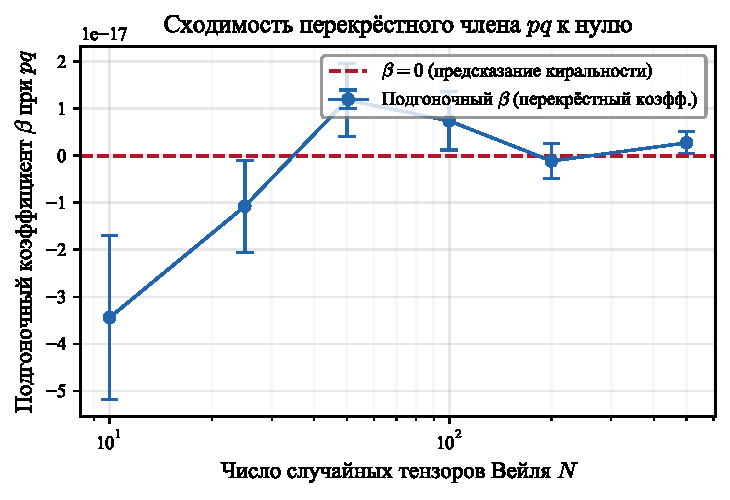
\includegraphics[width=0.7\textwidth]{../../analysis/figures/chirality/fig_pq_convergence_ru.pdf}
\caption{Сходимость подогнанного коэффициента перекрёстного члена $pq$
$\beta$ к нулю с ростом размера ансамбля.  Для каждого ансамбля из $N$
случайных тензоров Вейля вычисляется $\tr((\Omega^2)^2)$ и подгоняется
к $\alpha(p^2 + q^2) + \beta\,pq$.  Коэффициент $\beta$ согласуется с
нулём на уровне машинной точности ($|\beta| < 10^{-16}$) для всех размеров
ансамбля, подтверждая предсказание теоремы о киральности.  Планки
погрешностей обозначают стандартную ошибку подгонки методом наименьших
квадратов.}
\label{fig:pq-convergence}
\end{figure}


% ============================================================
\section{Заключение}
\label{sec:conclusions}
% ============================================================

Мы установили теорему о киральности для коэффициентов Сили--Де~Витта
оператора Дирака в четырёх измерениях: коммутация
$[\sigma^{rs}, \gamma_5] = 0$ делает спинорную кривизну $\Omega_{\mu\nu}$
блочно-диагональной, ядро теплопроводности разлагается на киральные секторы
с перекрёстным киральным соответствием (левый $\leftrightarrow$
антисамодуальный, правый $\leftrightarrow$ самодуальный), и все свёрнутые
коэффициенты $\tr(a_{2n})$ имеют нулевые перекрёстные члены между
$p = |C^+|^2$ и $q = |C^-|^2$.

На квартичном уровне (массовая размерность~8) это означает, что
спектральное действие порождает единственную эффективную структуру
$c(p^2 + q^2)$ с соотношением
$(C^2)^2 : ({}^{\ast}\!CC)^2 = 1{:}1$ точно.  В сочетании с тождеством
Кэли--Гамильтона (сводящим три инварианта Мольена к двум) и условием
киральности (сводящим два к одному) задача трёхпетлевой конечности
редуцируется от переопределённой системы к единственному условию на
соотношение.

Оставшийся вопрос --- уважают ли многопетлевые контрчлены структуру
спектрального действия --- разрешается отрицательно на основании
структурного аргумента и численных данных на конечных спектральных
тройках.  Строгая гипотеза о
спектральной перенормируемости (гипотеза~\ref{conj:spectral})
\emph{исключена на уровне структурного анализа}: пропагатор гравитона слеп к киральности (является
скаляром в поперечно-бесследовом секторе), и суммы по нескольким собственным значениям на
двух петлях и выше порождают перекрёстные члены $pq$, лежащие вне
пространства спектральных функций.  Это препятствие фундаментально для
гравитации и не возникает в случае Янга--Миллса~\cite{vanNuland:2021}, где
калибровочное поле входит как внутренняя флуктуация, сохраняющая
спектральную структуру.

Тем не менее утверждение о практической спектральной ультрафиолетовой
конечности (гипотеза~\ref{conj:practical}) сохраняется с сильной
количественной поддержкой: перекрёстные члены $pq$ подавлены множителем
$\alpha_C^3/(16\pi^2)^3 \approx 3{,}2 \times 10^{-10}$ относительно
ведущего действия, и первый петлевой порядок, на котором они становятся
физически значимыми, --- $L = 3$ (контрчлены размерности~8), поскольку
единственная структура $C^3$ на размерности~6 не различает $pq$ и
$p^2 + q^2$.

Результаты данной работы предоставляют алгебраический фундамент для
понимания трёхпетлевой структуры спектрального действия и точно
количественно определяют как область, так и пределы спектральной защиты
от ультрафиолетовых расходимостей.  Основные следствия для более широкой
программы: (1)~встроенная киральность спектрального действия снижает
эффективную размерность пространства контрчленов с двух до одного на уровне
разложения ядра теплопроводности, точно соответствуя единственному
доступному спектральному параметру; (2)~эта редукция не распространяется на
многопетлевые контрчлены из-за слепоты пропагатора гравитона к киральности;
(3)~нарушение количественно пренебрежимо, и спектральное действие
обеспечивает эффективную ультрафиолетовую конечность с точностью
$\sim 10^{-10}$.


% ============================================================
\section*{Благодарности}
% ============================================================

Все символьные результаты верифицированы
численно с точностью $\geq 12$ значащих цифр с использованием независимых
реализаций.


\appendix

% ============================================================
\section{Доказательство кирального соответствия символов 'т~Хоофта}
\label{app:thooft}
% ============================================================

Приведём явное вычисление, подтверждающее
утверждение~\ref{prop:thooft}.  Самодуальные символы 'т~Хоофта имеют вид:
\begin{alignat}{4}
  &\eta^1_{01} = 1, &\quad &\eta^1_{23} = 1, &\quad
  &\eta^2_{02} = 1, &\quad &\eta^2_{31} = 1, \notag\\
  &\eta^3_{03} = 1, &\quad &\eta^3_{12} = 1, &&&&
  \label{eq:eta-explicit}
\end{alignat}
(с $\eta^i_{ab} = -\eta^i_{ba}$, все остальные компоненты нулевые), а
антисамодуальные символы $\bar\eta^i$ отличаются знаком пространственных
компонент: $\bar\eta^i_{0j} = \eta^i_{0j}$,
$\bar\eta^i_{jk} = -\eta^i_{jk}$ для $j, k \in \{1,2,3\}$.

В киральном представлении с
$\gamma_5 = \mathrm{diag}(\mathbf{1}_2, -\mathbf{1}_2)$ генераторы
$4 \times 4$ спинорного представления $\sigma^{ab}$ разлагаются как
$\sigma^{ab} = \sigma^{ab}_L \oplus \sigma^{ab}_R$.
Свёртка:
\begin{alignat}{2}
  \eta^i_{ab}\,\sigma^{ab}_L &= 0 &\qquad &(i = 1,2,3), \notag\\
  \eta^i_{ab}\,\sigma^{ab}_R &\neq 0 &\qquad &(i = 1,2,3), \notag\\
  \bar\eta^i_{ab}\,\sigma^{ab}_L &\neq 0 &\qquad &(i = 1,2,3), \notag\\
  \bar\eta^i_{ab}\,\sigma^{ab}_R &= 0 &\qquad &(i = 1,2,3).
\end{alignat}
Это проверяется вычислением для каждого $i$ верхнего левого блока
$2 \times 2$ $P_L (\eta^i_{ab}\sigma^{ab}) P_L$ и нижнего правого блока
$2 \times 2$ $P_R (\eta^i_{ab}\sigma^{ab}) P_R$: первый обращается в
нуль, а второй является ненулевой линейной комбинацией матриц Паули.
Вычисление для $\bar\eta^i$ даёт противоположный результат.

Это устанавливает перекрёстное киральное соответствие: самодуальные компоненты
Вейля $C^+ \sim W^+_{ij}\eta^i\eta^j$ связываются с $\Omega^R$ (правыми
спинорами), а антисамодуальные компоненты
$C^- \sim W^-_{ij}\bar\eta^i\bar\eta^j$ связываются с $\Omega^L$ (левыми
спинорами).

\begin{figure}[ht]
\centering
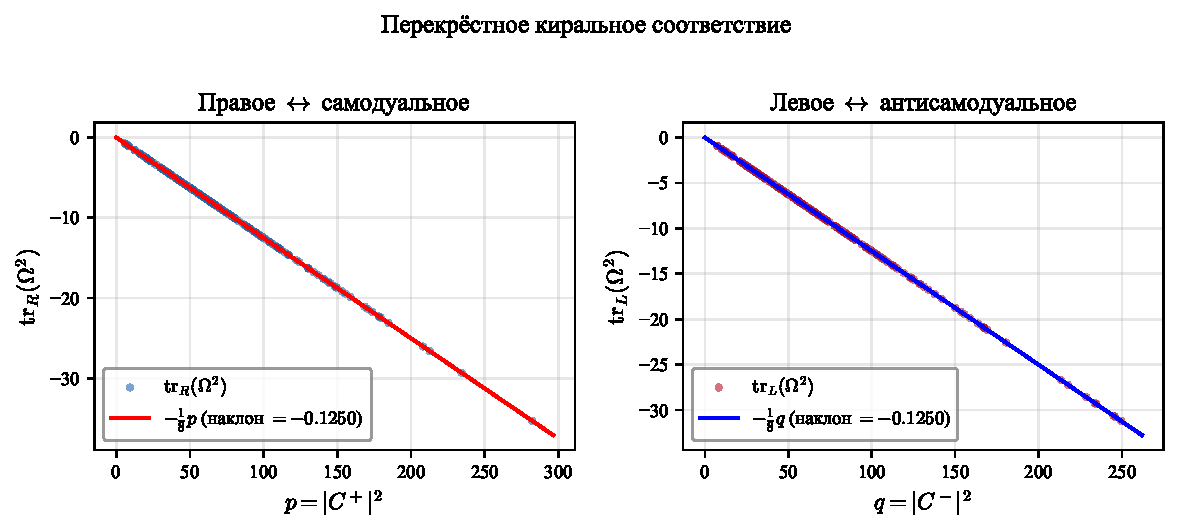
\includegraphics[width=0.95\textwidth]{../../analysis/figures/chirality/fig_crossed_chirality_ru.pdf}
\caption{Перекрёстное киральное соответствие, верифицированное на 200 случайных
тензорах Вейля.  Слева: $\tr_R(\Omega^2)$ линейно зависит от
$p = |C^+|^2$ с нулевой невязкой по~$q$.  Справа: $\tr_L(\Omega^2)$
линейно зависит от $q = |C^-|^2$ с нулевой невязкой по~$p$.
Наклоны составляют $-1/2$ в каждом киральном секторе, как предсказано
формулой~\eqref{eq:trOsq}.}
\label{fig:crossed-scatter}
\end{figure}


% ============================================================
\section{Вывод ряда Мольена}
\label{app:molien}
% ============================================================

Для полноты выведем P-чётный ряд
Мольена~\eqref{eq:molien}.

Тензор Вейля в $d = 4$ разлагается под действием $\mathrm{SO}(4)$ как:
\begin{equation}
  W = W^+ \oplus W^- \in \mathrm{Sym}_0^2(\mathbb{R}^3)
  \oplus \mathrm{Sym}_0^2(\mathbb{R}^3),
\end{equation}
где каждое $\mathrm{Sym}_0^2(\mathbb{R}^3)$ --- пространство бесследовых
симметричных матриц $3 \times 3$ (пятимерное).  Кольцо инвариантов одной
копии $\mathrm{Sym}_0^2$ относительно $\mathrm{SO}(3)$ имеет ряд
Мольена~\cite{Fulling:1992vm}:
\begin{equation}
  M(t) = \frac{1 + t^6}{(1 - t^2)(1 - t^3)(1 - t^4)}.
\end{equation}
Для двух копий с чётностью $W^+ \leftrightarrow W^-$ P-чётные
(<<скалярные>>) инварианты имеют ряд Мольена:
\begin{equation}
  P(t) = \frac{M(t)^2 + M(t^2)}{2}.
\end{equation}
Первый член подсчитывает все инварианты
$\mathrm{SO}(3) \times \mathrm{SO}(3)$ (произведение индивидуальных рядов
Мольена); второй осуществляет поправку на фактор-группу $\mathbb{Z}_2$
по чётности.  Разложение:
\begin{center}
\begin{tabular}{l|cccccccccc}
\toprule
Степень по $W$ & 0 & 2 & 3 & 4 & 5 & 6 & 7 & 8 & 9 & 10 \\
\midrule
$P(\text{степ.})$ & 1 & 1 & 1 & 3 & 2 & 7 & 5 & 13 & 12 & 23 \\
\bottomrule
\end{tabular}
\end{center}
На степени~4 (квартичные по Вейлю): $P_4 = 3$ P-чётных
инварианта, что подтверждает результат~\eqref{eq:three-invariants}.

При сопоставлении петлевых порядков (массовая размерность $= 2L + 2$ для
$L$-петлевого контрчлена на массовой оболочке в Риччи-плоской гравитации,
следовательно степень $L + 1$ по тензору Вейля), $L = 3$ соответствует
степени~4, давая 3 инварианта против 1 спектрального параметра.  После
редукции Кэли--Гамильтона ($3 \to 2$) и киральной редукции ($2 \to 1$)
система становится определённой.


\section*{Финансирование}

Работа не имела внешнего финансирования.

\section*{Конфликт интересов}

Автор заявляет об отсутствии конфликта интересов.

\bibliographystyle{unsrtnat}
\bibliography{../references/sct_chirality}


\end{document}
